% TEMPLATE for Usenix papers, specifically to meet requirements of
%  USENIX '05
% originally a template for producing IEEE-format articles using LaTeX.
%   written by Matthew Ward, CS Department, Worcester Polytechnic Institute.
% adapted by David Beazley for his excellent SWIG paper in Proceedings,
%   Tcl 96
% turned into a smartass generic template by De Clarke, with thanks to
%   both the above pioneers
% use at your own risk.  Complaints to /dev/null.
% make it two column with no page numbering, default is 10 point

% Munged by Fred Douglis <douglis@research.att.com> 10/97 to separate
% the .sty file from the LaTeX source template, so that people can
% more easily include the .sty file into an existing document.  Also
% changed to more closely follow the style guidelines as represented
% by the Word sample file. 

% Note that since 2010, USENIX does not require endnotes. If you want
% foot of page notes, don't include the endnotes package in the 
% usepackage command, below.

\documentclass[letterpaper,twocolumn,10pt]{article}
\usepackage{usenix,epsfig,endnotes}
\usepackage{listings}
\usepackage{xspace}
\usepackage{xcolor}

\definecolor{codegreen}{rgb}{0,0.6,0}
\definecolor{codegray}{rgb}{0.5,0.5,0.5}
\definecolor{codepurple}{rgb}{0.58,0,0.82}
\definecolor{backcolour}{rgb}{0.95,0.95,0.92}

\lstdefinestyle{mystyle}{
    backgroundcolor=\color{backcolour},   
    commentstyle=\color{codegreen},
    keywordstyle=\color{magenta},
    numberstyle=\tiny\color{codegray},
    stringstyle=\color{codepurple},
    basicstyle=\ttfamily\footnotesize,
    breakatwhitespace=false,         
    breaklines=true,                 
    captionpos=b,                    
    keepspaces=true,                 
    numbers=left,                    
    numbersep=5pt,                  
    showspaces=false,                
    showstringspaces=false,
    showtabs=false,                  
    tabsize=2
}

\lstset{style=mystyle}

\newcommand{\work}{\mbox{\textsc{RADAR}}\xspace}

\begin{document}

%don't want date printed
\date{}

%make title bold and 14 pt font (Latex default is non-bold, 16 pt)
\title{\Large \bf \work: Ransomware Auto-Detection At Runtime}

\author{
{\rm Kimia Saedi}\\
ks152@rice.edu
\and
{\rm Weijie Huang}\\
wh31@rice.edu
}

\maketitle

% Use the following at camera-ready time to suppress page numbers.
% Comment it out when you first submit the paper for review.
% \thispagestyle{empty}


\subsection*{Abstract}

Ransomware attacks have been a huge threat for personal and business data safety. 
The malicious person usually launches denial-of-access attacks to user files to request for ransom payments.
As the number of victims increases with the year, it is important to introduce detection methods to avoid property loss in the early stage.
Recent state-of-art works tend to utilize Cuckoo Sandbox for information gathering.
However, Cuckoo-based solutions can only capture API-granularity data, which might miss the characteristics of memory (usually heap) access behaviors.
In this project, we will propose \work that integrates Intel’s dynamic binary instrumentation framework (Pin) as well to collect more comprehensive data.
The runtime information will be classified by a supervised learning trained model.
We will evaluate the detection quality of \work by the end of this project.

\section{Introduction}

Ransomware is a type of malicious software (i.e., malware) that usually blocks users from controlling the computer or accessing files to request ransom payments.
It often uses hard-to-crack methods to encrypt files, forcing victims to pay to regain access to their data.
WannaCry,~\cite{wannacry_2017} one of the most famous ransom attacks in recent times, has caused incalculable damage worldwide, which impacted countless computers in companies, organizations and governments.
According to a recent survey,~\cite{cybereason_2022} 73\% of the cybersecurity professionals reported that their organization was attacked by ransomware, which is 33\% more than the statistics in 2021.
Moreover, 63\% of the respondents reported that the attackers might have been lurked in their networks for up to six months, which emphasizes the significance of early detection against potentially malicious behavior.

In recent years, researchers have proposed several patterns, metrics and detection algorithms to identify and/or capture ransomware features.~\cite{Chen2019AutomatedRB, 8051108, Morat2018RansomwareED, Verma2018DefiningAM}
Typically, such features can be obtained by analyzing the interaction behavior between a program and the operating system.
Most state-of-art works utilize Cuckoo Sandbox,~\cite{CuckooSS} an open-source sandbox tool with powerful logging capabilities, to record and analyze invocations of system APIs.
% However, Cuckoo can only capture high-level interactions, while memory-based operations may also be essential for ransomware identification.
However, Cuckoo can only capture high-level interactions, which seems coarse-grained because some malicious operations might utilize memory directly for attacks.
It is intuitive to capture more detailed behavior (e.g. heap usage) to obtain more complete runtime information for identification.
In this project, we aim to propose \work, an automated ransomware detection tool at run time.
We will utilize Pin,~\cite{pin} a robust binary instrumentation tool for x86/64 machines, to assist Cuckoo with information gathering.
Then we will propose a supervised learning model to detect ransomware-like behaviors from the collected runtime features.
We will evaluate the model with both ransomware and ordinary programs to test the model accuracy.

\section{Background}

A malware detector typically uses static and dynamic analysis techniques to evaluate a sample's behavior and risks. Static analyses are done before execution. Considering that, they struggle to analyze obfuscated code which is the case in most threats. Dynamic analyses have shown better results for malware detection because they track the malware behavior and activities by executing the malware sample. In this work, we use data collected from Cuckoo Sandbox plus Pin in order to run dynamic analysis. 

UNVEIL~\cite{197235} is a novel dynamic analysis system for detecting ransomware attacks and recognizing their behaviors. UNVEIL is a rule-based ransomware detector that monitors access patterns in terms of I/O traces and alarms on ransomware-like behavior while our approach is more general purpose in this work we propose a data-driven automated ransomware detector based on machine learning techniques however it is possible to turn it into a powerful Intrusion Detection System (IDS) in future attempts.

\section{Methodology}

In this work we aim at, first, finding the most indicative characteristics of ransomware attacks exploiting their dynamic behavior, second, using the extracted feature vector of labeled attack and benign traces we then explore the most effective supervised learning algorithms to detect such malware.
For that we make use of Cuckoo Sandbox reports that generate the high-level data including static information such as imported DLLs, compilation time, etc., and dynamic information such as sequence of processes, API calls and their frequency also some behaviour signatures in form of flags combined with the Pin trace data that comprises low-level memory access patterns. After data collection phase for each sample run we input the resulted dataset into a data mining tool called WEKA~\cite{weka} for benchmarking the machine learning algorithims with measuring the accuracy metrics. 
Having that in mind we hypothesis that with regard to the sequential nature of program traces the Attention-based solution might be the most effective technique to charactrize malwares.

% \subsection{Cuckoo Tracing}

% TODO @Kimia

\subsection{Pin Tracing}

\begin{figure}
    \centering
    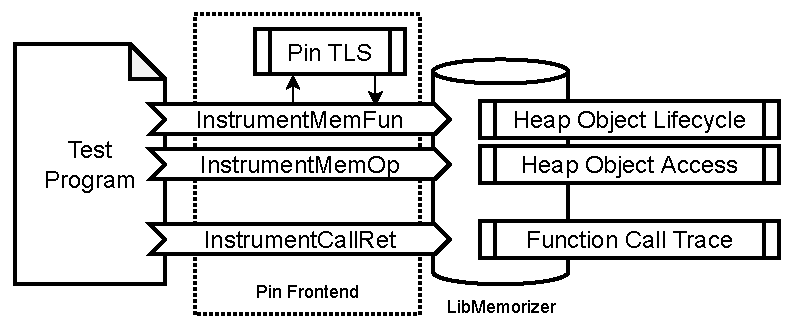
\includegraphics[width=\linewidth]{pin.pdf}
    \caption{Pin Tracing Overview}
    \label{fig:pin}
\end{figure}

For memory access patterns, we use Pin as the frontend to instrument the target program, then pass the runtime information to the backend, \textit{LibMemorizer}.
Pin is a safe and powerful instrument tool to insert JIT code dynamically.
It provides PinCRT to support essential parts of C/C++ standard library to eliminate dependency to the host system.
The structure of the whole process is shown in Figure~\ref{fig:pin}.

\subsubsection{Pin Frontend}

First we use Pin to hook every entrypoint of heap-relevant functions such as \texttt{malloc}, \texttt{calloc} and \texttt{realloc}.
Pin can obtain the function arguments right before the call site and get the return value right after.
However, for \texttt{malloc} calls, we need to capture both the arguments and the return value (i.e. the pointer to the heap object) to record the object creation.
Observing that the target program might be multithreaded, we use Pin's thread-local storage API to store the arguments in advance.
After the function returns, the stored arguments can be passed to the backend with the corresponding return pointer.
When \texttt{free} is called, the corresponding pointer will be directly sent to the backend to invalidate the object.

After hooking the heap objects, we instrument every load/store instructions to record accesses to the alive objects.
However, most of these instructions are accessing local (stack) variables/objects, which need to be filtered out.
We leave this operation to the backend for future compatibility to track stack accesses and/or identify stack overflows.

The above operations can only record the instruction addresses without further symbol information. 
Pin has provided the symbol parsing functionalities, so it is intuitive to track function call traces to grasp the function symbols that might help with analysis.
There are three types of unconditional control flow redirections that might represent control flow: \textit{call}, \textit{return} and \textit{jump}.
We instrumented all these instructions to pass the address and symbol information to the backend.

\subsubsection{LibMemorizer}

\textit{LibMemorizer} is a standalone library to record and store program's runtime data.
It is now compatible on Windows and Linux machines and can support both native library and PinCRT.

For heap objects, we will store all data (even the object is freed) into a linked list.
For those ``alive'' objects (i.e., not freed yet), we maintain a lookup table to index the addresses.
When an instruction tries to access the heap, we can quickly locate the corresponding object, then add an access entry with access type and timestamp.
The timestamp is useful to determine the access frequency on the heap.
For the instructions accessing the stack, because of the address consistency of the user stack, we can easily filter them out by comparing the target address with an approximation of the stack pointer.
In the end, all heap object information will be logged.

As for control flows, we maintain a shadow stack to record the calling relationship between functions.
Because PinCRT does not provide thread-local storage interfaces to third-party libraries, we implemented a simple map that takes the thread ID as the key to access thread-sepecific stacks.
Moreover, the library logs the calling information so that the call trace can be collected for further processing.

\section{Progress}

So far the basic functionalities of Pin and \textit{LibMemorizer} are finished.
The workflow has been successfully tested on Linux and Windows with simple test programs.
The source code for the test program is shown in Appendix~\ref{app:test}.

We can read the heap object information from the log outputs:

\small
\begin{verbatim}
Sobj#0 alloc_type=0
  alloc'd @0x7f1c4ecd796c, size=64
  freed @0x7f1c4ecd7990
  accesses:
    type=1, time=1511350, pinst=0x7f1c3d1a04fa
    type=1, time=1511352, pinst=0x7f1c3d1a0530
    type=0, time=1523590, pinst=0x7f1c3d1a1512
    type=0, time=1526048, pinst=0x7f1c3d1a184c
    type=0, time=1527339, pinst=0x7f1c3d1a1e38
    type=0, time=1527340, pinst=0x7f1c3d1a1e7a
    type=0, time=1528188, pinst=0x7f1c3d19f943
    type=1, time=1528190, pinst=0x7f1c3d19fa76
    type=1, time=1528191, pinst=0x7f1c3d19fb1d
Sobj#1 alloc_type=0
  alloc'd @0x7f1c4ecd7990, size=128
  va @0x55d4f4e91490
  accesses:
    type=0, time=1533699, pinst=0x7f1c3d1a28f2
    type=0, time=1533700, pinst=0x7f1c3d1a2959
Sobj#2 alloc_type=0
  alloc'd @0x7f1c4ecd796c, size=16
  freed @0x7f1c3d19f152
  accesses:
    type=1, time=1537418, pinst=0x7f1c3d1a2dd1
    type=0, time=1537419, pinst=0x7f1c3d1a2dfe
    type=1, time=1537419, pinst=0x7f1c3d1a2e56
\end{verbatim}
\normalsize

Similarly we have logs for function calls.
The result file is too large so we do not put the content into this report.

% TODO @Kimia

% \section{Project Plan}

% We divide the project into three phases:

% \paragraph{Phase 1: Data collection.}

% By Oct 21, we will figure out the workflow for raw runtime data, which consists of two parts: Cuckoo logs and instrumented outputs.
% The former one is trivial. For the latter part, We will insert function calls to a runtime library, \textit{LibMemorizer}, to record memory allocations/deallocations/accesses. The runtime data will be dumped into a file for later analysis.

% To better observe the program behavior, we need to grasp the information of the function caller.
% We will carry out experiments on Windows, so it is essential to develop an auxiliary tool to parse the symbol table.
% Similar to ELF, Windows executable files have a header structure to identify the file layout.
% This way, we can identify the specific functions who perform probably malicious operations.

% \paragraph{Phase 2: Feature extraction.} By Oct 31, we will count the collected data and extract the characteristics that could be fed to the network model.
% In other words, we will provide a ransomware behavior dataset for model detection.
% Then, we will propose and build the network to learn the ransomware patterns from the characteristics by Nov 15.

% \paragraph{Phase 3: Training and evaluation.} After building the dataset and network, we will train the model and test the effectiveness of the detection.
% We will try to make efforts to optimize the model performance.
% In the end, we might produce a full workflow for \work.



{\footnotesize \bibliographystyle{acm}
\bibliography{sample}}

\appendix

\section{Test Program Source Code}
\label{app:test}

\begin{lstlisting}[language=c]
#include <stdlib.h>
#include <string.h>

void fun()
{
    int* p = (int*)calloc(sizeof(int), 100);
    p[0] = 1;
    p[99] = p[1];
    free(p);
}

int main()
{
    char s[] = "Hello world";
    void* p = malloc(64);
    fun();
    strcpy((char*)p, s);
    char* news = realloc(p, 128);
    if (news[4] == news[7]) {
        long* pl = realloc(NULL, 2*sizeof(long));
        pl[0] = pl[1] = 1;
        free(pl);
    }
    char _ = news[128];
    // free(news);
    return 0;
}
\end{lstlisting}
% \theendnotes

\end{document}







